\section{Results}
\label{sec:results}

\subsection{The three models of the prediction in the stress windows}
\label{sec:results-main}

\Cref{tab:main-results} gives, for HS-250, GARCH-t and filtered historical simulation, the hits of the unwrapped and the wrapped model in each stress window and level, the Kupiec and conditional coverage p-values, the independence p-value of the wrapped model and the change of the mean score with its bootstrap interval. The wrapped model has fewer hits than the unwrapped one in 16 of the 18 rows, and equal in the other two (FHS in the pandemic window at the 1\% level and in the rates window at 1\%, where the unwrapped model already passes). The largest reductions are those of historical simulation: in the financial crisis window the unwrapped model has \hitUHsTwoFiftyOneEqCrisis{} hits at the 1\% level against \hitWHsTwoFiftyOneEqCrisis{} wrapped, with \nDaysEqCrisis{} days expected to give 5.0, and at the 2.5\% level \hitUHsTwoFiftyTwoHalfEqCrisis{} against \hitWHsTwoFiftyTwoHalfEqCrisis{}. The Kupiec p-value of the wrapped historical simulation in that window is \kupWHsTwoFiftyOneEqCrisis{} at 1\%, below 0.05: the wrapped model still fails the unconditional test at the 1\% level, and it passes at 2.5\% (\kupWHsTwoFiftyTwoHalfEqCrisis{}, conditional coverage \ccWHsTwoFiftyTwoHalfEqCrisis{}). In the pandemic window, historical simulation stays below the bar at both levels after the wrap (Kupiec p-values \kupWHsTwoFiftyOneEqCovid{} and \kupWHsTwoFiftyTwoHalfEqCovid{}), with 6 and 7 hits in 104 days against 1.0 and 2.6 expected; the crash of March 2020 comes with the level already at the lower edge of the band (\clipHsTwoFiftyOneEqCovid{} days at the edge at the 1\% level).

\begin{table*}[htbp]
\centering
\small
\caption{Unwrapped (U) and wrapped (W) value at risk of three ladder models in the three stress windows of C11, at tail levels 1\% and 2.5\%: hits, the hit rate of the wrapped model with its 95\% Wilson interval, the p-values of the Kupiec and conditional coverage (CC) tests, the Christoffersen independence p-value of the wrapped model and the relative change of the mean FZ0 score with a 95\% moving-block bootstrap interval (positive is worse). The windows hold 504, 104 and 249 forecast days.}
\label{tab:main-results}
\begin{adjustbox}{max width=\textwidth}
\begin{tabular}{llrrlllll}
\toprule
Window & Model & Level (\%) & Hits U & Hits W (rate \%; 95\% Wilson) & Kupiec $p$ U / W & CC $p$ U / W & Indep. $p$ W & FZ0 change [95\% CI] \\
\midrule
Equity 2007--09 & HS-250 & 1 & 19 & 11 (2.2; 1.2--3.9) & $<0.001$ / 0.021 & $<0.001$ / 0.055 & 0.483 & \relax -17.2\% [-59.9\%, -1.3\%] \\
Equity 2007--09 & HS-250 & 2.5 & 36 & 17 (3.4; 2.1--5.3) & $<0.001$ / 0.233 & $<0.001$ / 0.271 & 0.275 & \relax -14.3\% [-40.3\%, -1.8\%] \\
Equity 2007--09 & GARCH-t & 1 & 16 & 6 (1.2; 0.5--2.6) & $<0.001$ / 0.677 & $<0.001$ / 0.853 & 0.703 & \relax -4.2\% [-12.4\%, +1.8\%] \\
Equity 2007--09 & GARCH-t & 2.5 & 31 & 14 (2.8; 1.7--4.6) & $<0.001$ / 0.695 & $<0.001$ / 0.620 & 0.371 & \relax -3.6\% [-10.5\%, +1.5\%] \\
Equity 2007--09 & FHS & 1 & 13 & 7 (1.4; 0.7--2.8) & 0.003 / 0.407 & 0.009 / 0.643 & 0.657 & \relax -3.2\% [-10.8\%, +1.7\%] \\
Equity 2007--09 & FHS & 2.5 & 24 & 14 (2.8; 1.7--4.6) & 0.004 / 0.695 & 0.005 / 0.620 & 0.371 & \relax -1.7\% [-6.5\%, +2.1\%] \\
Equity 2020 & HS-250 & 1 & 8 & 6 (5.8; 2.7--12.0) & $<0.001$ / 0.001 & $<0.001$ / 0.002 & 0.327 & \relax -168.7\% [-1274.5\%, +13.0\%] \\
Equity 2020 & HS-250 & 2.5 & 13 & 7 (6.7; 3.3--13.2) & $<0.001$ / 0.022 & $<0.001$ / 0.055 & 0.468 & \relax -631.7\% [-2271.3\%, +17.5\%] \\
Equity 2020 & GARCH-t & 1 & 3 & 2 (1.9; 0.5--6.7) & 0.116 / 0.401 & 0.265 / 0.676 & 0.778 & \relax +3.0\% [-3.4\%, +28.2\%] \\
Equity 2020 & GARCH-t & 2.5 & 6 & 5 (4.8; 2.1--10.8) & 0.067 / 0.180 & 0.116 / 0.185 & 0.209 & \relax -2.2\% [-24.6\%, +5.8\%] \\
Equity 2020 & FHS & 1 & 2 & 2 (1.9; 0.5--6.7) & 0.401 / 0.401 & 0.676 / 0.676 & 0.778 & \relax +3.4\% [+1.1\%, +10.3\%] \\
Equity 2020 & FHS & 2.5 & 5 & 4 (3.8; 1.5--9.5) & 0.180 / 0.415 & 0.316 / 0.610 & 0.570 & \relax +1.5\% [-0.2\%, +4.5\%] \\
Rates 2022 & HS-250 & 1 & 8 & 4 (1.6; 0.6--4.1) & 0.005 / 0.377 & 0.016 / 0.644 & 0.754 & \relax -5.8\% [-24.9\%, +3.5\%] \\
Rates 2022 & HS-250 & 2.5 & 14 & 8 (3.2; 1.6--6.2) & 0.007 / 0.490 & 0.011 / 0.624 & 0.495 & \relax -3.3\% [-10.5\%, +1.3\%] \\
Rates 2022 & GARCH-t & 1 & 6 & 4 (1.6; 0.6--4.1) & 0.058 / 0.377 & 0.147 / 0.644 & 0.754 & \relax -0.2\% [-7.5\%, +4.5\%] \\
Rates 2022 & GARCH-t & 2.5 & 14 & 8 (3.2; 1.6--6.2) & 0.007 / 0.490 & 0.011 / 0.624 & 0.495 & \relax -0.3\% [-3.0\%, +1.6\%] \\
Rates 2022 & FHS & 1 & 5 & 5 (2.0; 0.9--4.6) & 0.160 / 0.160 & 0.343 / 0.343 & 0.685 & \relax +0.9\% [-3.4\%, +3.9\%] \\
Rates 2022 & FHS & 2.5 & 12 & 7 (2.8; 1.4--5.7) & 0.037 / 0.758 & 0.065 / 0.801 & 0.555 & \relax -0.3\% [-3.0\%, +1.4\%] \\
\bottomrule
\end{tabular}
\end{adjustbox}
\end{table*}


\Cref{fig:hit-rates} shows the same results as hit rates with their Wilson intervals: the wrapped hit rate is closer to the target than the unwrapped one, or equal to it, in every cell. The intervals are wide, because the windows hold between 2 and 36 hits in each cell of the unwrapped models and between 2 and 17 in the wrapped ones: the interval of the wrapped hit rate of GARCH-t at the 1\% level in the crisis window is 0.5\% to 2.6\%, which contains the target. \Cref{fig:level-paths} shows what the wrapper did. The working level of historical simulation falls to the band edge on \clipHsTwoFiftyOneEqCrisis{} days of the crisis window and on \clipHsTwoFiftyOneRates{} days of the rates window at the 1\% level and recovers slowly between clusters, as \cref{eq:cluster-drop} predicts: a single hit at the 1\% level needs about 100 quiet days to be undone. The level of GARCH-t, whose own volatility filter follows the crisis, reaches the edge on \clipGarchTOneEqCrisis{} days in the crisis window and on none in the pandemic window, where its minimum level is 0.0045.

\begin{figure}[htbp]
\centering
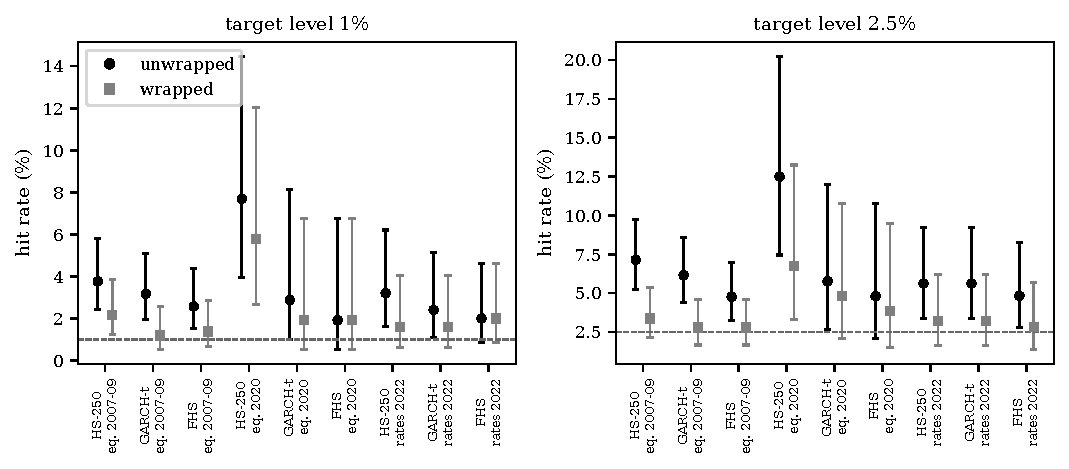
\includegraphics[width=\textwidth]{hit-rates}
\caption{Hit rate of the unwrapped (circles) and wrapped (squares) value at risk of HS-250, GARCH-t and FHS in the three stress windows, at the 1\% (left) and 2.5\% (right) target levels, with 95\% Wilson intervals; the dashed line is the target.}
\label{fig:hit-rates}
\end{figure}

\begin{figure}[htbp]
\centering
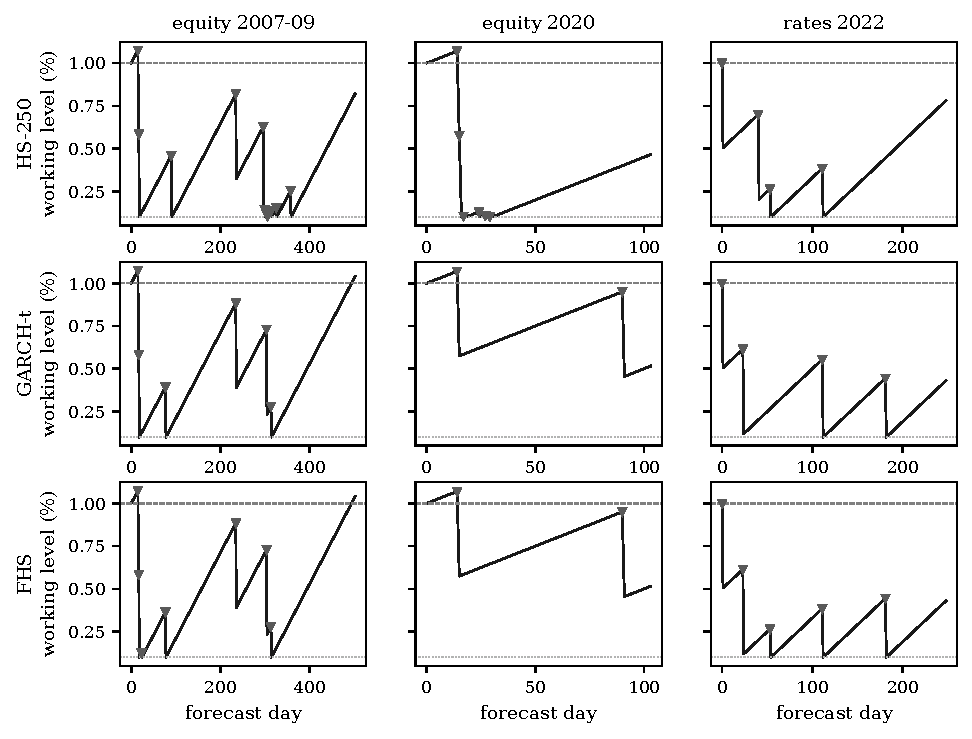
\includegraphics[width=\textwidth]{level-paths}
\caption{Working level of the wrapper at the 1\% target for HS-250, GARCH-t and FHS (rows) in the three stress windows (columns): the level in percent by forecast day, the days of a hit of the wrapped model marked by triangles, the target as a dashed line and the lower edge of the band as a dotted line.}
\label{fig:level-paths}
\end{figure}

\subsection{Whether the hypotheses held}
\label{sec:results-hypotheses}

\Cref{tab:hypotheses} applies the rule of H1 to the six cells of the hypothesis and to the other fourteen cells of the ten wrapped models. H1 holds in all \hypCells{} cells of HS-250, GARCH-t and FHS: the wrapped models gain \hypExtraTotal{} stress-window passes in all (HS-250 one window at 1\% and two at 2.5\%, GARCH-t one and two, FHS one and two), and the worst change of the mean score in any stress window is \hypWorstFz\%, below the 5\% tolerance. H2 does not occur: the independence p-values of the wrapped models in the crisis window run from \indMin{} to \indMax{}, and \indFails{} of the six are below 0.05. The hypothesis holds as a whole as it was written, with the engine's Kupiec and conditional coverage tests as the pass rule. Those tests accept wrapped runs more easily than unwrapped ones (\cref{sec:results-dispersion}); tested on coverage alone against the null of the wrapped count, H1 holds in \dispCHoneGainCal{} of the \hypCells{} cells, the cell that falls being \dispCHoneLost. The statement carries a qualification that the table makes visible: of the \hypExtraTotal{} extra passes, none comes from the pandemic window for HS-250, and the extra passes of GARCH-t and FHS are in the crisis window (and in the rates window at the 2.5\% level), where the unwrapped Kupiec p-values are 0.004 or below in the crisis window and at most 0.037 in the rates window.

Applied to the ten models, the rule holds in \tenCellsHold{} of \tenCells{} cells. The cell that fails is \tenNoGainCells{}: it gains no window, although its hit rate improves, and the level sits at the band edge on \clipDnRollingOneEqCrisis{} days of the crisis window, so the band, not the update, limits what the model can reach. Across the ten models the wrapped runs pass \tenPassAci{} of \tenRuns{} cells against \tenPassUnw{} unwrapped by the engine's tests (\dispCWrapCal{} against \dispCUnwExact{} on coverage alone, with each count tested against its own null; \cref{sec:results-dispersion}), no wrapped run fails the independence test in the stress windows (and none in the \tenIndRunsAll{} runs of all six windows), and the mean absolute distance of the hit rate from its target falls from \tenHitDevUnw{} to \tenHitDevAci{} percentage points.

\begin{table}[htbp]
\centering
\small
\caption{The prediction for each of the ten wrapped ladder models and two tail levels: windows passed (Kupiec and conditional coverage both at least 0.05) out of the three stress windows, unwrapped (U) and wrapped (W), the extra windows gained, the worst relative FZ0 change in any stress window, the independence p-value of the wrapped model in equity 2007--09 and whether the prediction holds. The first six rows are the models of the prediction as stated; the other rows apply the same rule to the remaining models.}
\label{tab:hypotheses}
\begin{adjustbox}{max width=\textwidth}
\begin{tabular}{lrrrrrrl}
\toprule
Model & Level (\%) & Windows passed U & Windows passed W & Extra & Worst FZ0 change & Indep. $p$ W, 2007--09 & Holds \\
\midrule
HS-250 & 1 & 0 & 1 & 1 & \relax -5.8\% & 0.483 & yes \\
HS-250 & 2.5 & 0 & 2 & 2 & \relax -3.3\% & 0.275 & yes \\
HS-500 & 1 & 0 & 1 & 1 & \relax -0.9\% & 0.483 & yes \\
HS-500 & 2.5 & 0 & 2 & 2 & \relax -5.0\% & 0.248 & yes \\
AWHS & 1 & 0 & 1 & 1 & \relax -1.1\% & 0.483 & yes \\
AWHS & 2.5 & 1 & 3 & 2 & \relax -0.4\% & 0.305 & yes \\
Delta-normal & 1 & 0 & 0 & 0 & \relax -21.9\% & 0.935 & no \\
Delta-normal & 2.5 & 0 & 1 & 1 & \relax -10.0\% & 0.836 & yes \\
EWMA & 1 & 1 & 2 & 1 & \relax -0.0\% & 0.657 & yes \\
EWMA & 2.5 & 1 & 2 & 1 & \relax +0.3\% & 0.371 & yes \\
GARCH-t & 1 & 2 & 3 & 1 & \relax +3.0\% & 0.703 & yes \\
GARCH-t & 2.5 & 1 & 3 & 2 & \relax -0.3\% & 0.371 & yes \\
GJR-t & 1 & 2 & 3 & 1 & \relax +2.9\% & 0.703 & yes \\
GJR-t & 2.5 & 1 & 3 & 2 & \relax -0.9\% & 0.337 & yes \\
EGARCH-t & 1 & 2 & 3 & 1 & \relax -0.2\% & 0.567 & yes \\
EGARCH-t & 2.5 & 0 & 3 & 3 & \relax -0.8\% & 0.248 & yes \\
FHS & 1 & 2 & 3 & 1 & \relax +3.4\% & 0.657 & yes \\
FHS & 2.5 & 1 & 3 & 2 & \relax +1.5\% & 0.371 & yes \\
Conditional EVT & 1 & 2 & 3 & 1 & \relax +4.3\% & 0.703 & yes \\
Conditional EVT & 2.5 & 1 & 3 & 2 & \relax +1.9\% & 0.371 & yes \\
\bottomrule
\end{tabular}
\end{adjustbox}
\end{table}


\subsection{The score of the pair}
\label{sec:results-score}

The change of the mean score is the second condition of H1, and \cref{fig:fz0-change} shows it for the ten models with the bootstrap intervals. The change is negative (the wrapped pair scores better) in most cells, with a mean of \tenMeanFz\% over the \tenRuns{} cells, and the largest improvement is that of HS-500 at the 2.5\% level in the pandemic window (\tenBestFz\%), where the unwrapped VaR sits near the calm past on a sudden crash. The largest positive changes are those of the filtered models and the extreme-value model at the 1\% level (\worstFzGarchTOne\% for GARCH-t, \worstFzFhsOne\% for FHS, \worstFzEvtMfOne\% for the extreme-value model), all below the 5\% tolerance, and their intervals contain zero in most windows (\cref{fig:fz0-change}); the one exception in the table is FHS in the pandemic window at the 1\% level, with an interval of +1.1\% to +10.3\%, whose upper end is over the tolerance. The intervals of the historical-simulation cells in the pandemic window run from $-1{,}274.5\%$ to $+13.0\%$ at the 1\% level and from $-2{,}271.3\%$ to $+17.5\%$ at 2.5\% (\cref{tab:main-results}) because the unwrapped score is close to zero on 104 days and its relative change is unstable; the absolute differences are the better guide there.

\begin{figure}[htbp]
\centering
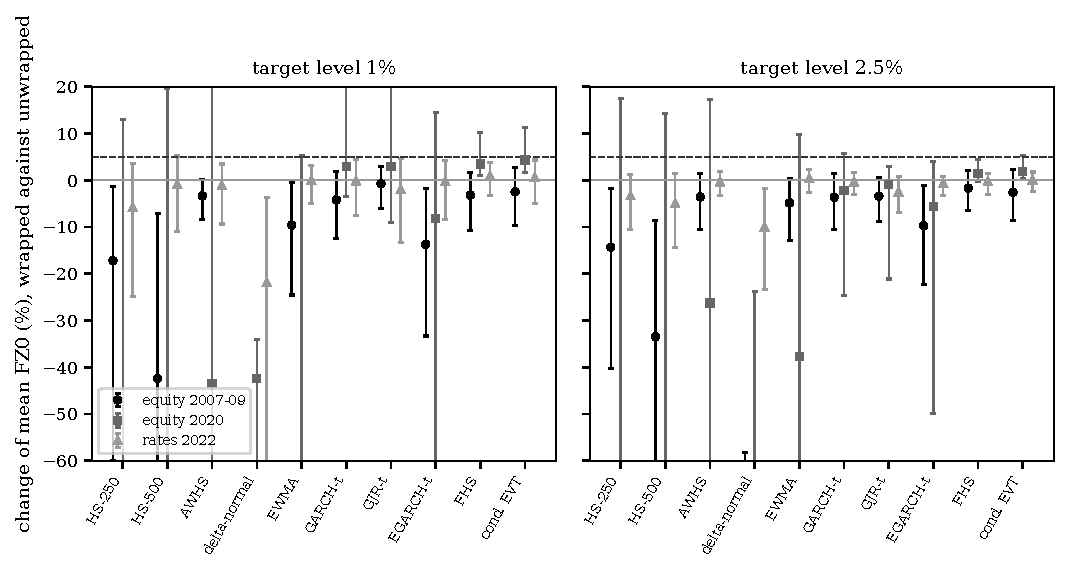
\includegraphics[width=\textwidth]{fz0-change}
\caption{Relative change of the mean FZ0 score of the wrapped against the unwrapped model for the ten wrapped ladder models in the three stress windows, at the 1\% (left) and 2.5\% (right) levels, with 95\% moving-block bootstrap intervals; the dashed line is the 5\% tolerance and values below zero are improvements.}
\label{fig:fz0-change}
\end{figure}

The ES stays understated: the mean $Z_2$ of the ten models in the stress windows is \tenMeanZtwoUnw{} unwrapped and \tenMeanZtwoAci{} wrapped, a halving of the shortfall that leaves it far from zero. The wrapper repairs the VaR and carries the ES along, but it does not make the ES correct, which is the content of \cref{prop:es} for tails that are not Pareto.

\subsection{The ladder as a whole}
\label{sec:results-ladder}

\Cref{tab:ladder-context} and \cref{fig:ladder-pass} put the wrapped models back among the eighteen. In the crisis window no model of the ladder passes at either level as the ladder runs. With the three models of H1 replaced by their wrapped versions, \ladThreeEqCrisisOne{} pass at the 1\% level and \ladThreeEqCrisisTwoHalf{} at 2.5\%; with the ten wrapped models, \ladTenEqCrisisOne{} and \ladTenEqCrisisTwoHalf{} of the eighteen. In the pandemic window the count rises from \ladUEqCovidOne{} to \ladTenEqCovidOne{} at 1\% and from \ladUEqCovidTwoHalf{} to \ladTenEqCovidTwoHalf{} at 2.5\%; in the rates window from \ladURatesOne{} to \ladTenRatesOne{} and from \ladURatesTwoHalf{} to \ladTenRatesTwoHalf{}. The eight models that are not wrapped (three that give no ES, five fitted for one level) keep their unwrapped results in these counts, so the figures understate what a wrap of every model would give. The counts of the wrapped models are the engine's, and inherit the lenience measured in \cref{sec:results-dispersion}: they show how many models the supervisor's tests would pass, not how many are correctly sized.

\begin{table}[htbp]
\centering
\small
\caption{The eighteen-model ladder of C11 in the three stress windows: how many models pass the Kupiec and conditional coverage tests (both p at least 0.05) as the ladder runs, with the three models of the prediction replaced by their wrapped versions, and with the ten level-parametric models replaced by their wrapped versions.}
\label{tab:ladder-context}
\begin{adjustbox}{max width=\textwidth}
\begin{tabular}{lrrrrr}
\toprule
Window & Level (\%) & Ladder models & Pass, none wrapped & Pass, three wrapped & Pass, ten wrapped \\
\midrule
Equity 2007--09 & 1 & 18 & 0 & 2 & 6 \\
Equity 2007--09 & 2.5 & 18 & 0 & 3 & 9 \\
Equity 2020 & 1 & 18 & 5 & 5 & 5 \\
Equity 2020 & 2.5 & 18 & 6 & 6 & 8 \\
Rates 2022 & 1 & 18 & 10 & 11 & 13 \\
Rates 2022 & 2.5 & 18 & 5 & 8 & 13 \\
\bottomrule
\end{tabular}
\end{adjustbox}
\end{table}


\begin{figure}[htbp]
\centering
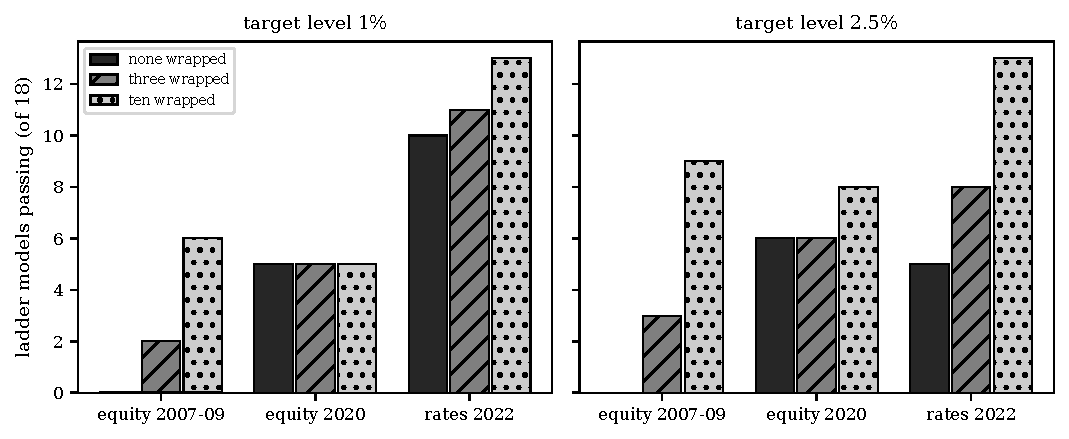
\includegraphics[width=\textwidth]{ladder-pass}
\caption{Number of the eighteen ladder models that pass the Kupiec and conditional coverage tests in each stress window at the 1\% (left) and 2.5\% (right) levels: as the ladder runs (dark bars), with the three models of the hypothesis wrapped (hatched bars) and with the ten level-parametric models wrapped (light bars).}
\label{fig:ladder-pass}
\end{figure}

\subsection{Against other recalibrations}
\label{sec:results-comparators}

\Cref{tab:comparators} and \cref{fig:methods-pass} compare the wrapper with the two recalibrations that act on the finished VaR, run on the same VaR and the same ES (both scaled by the same factor) of the same ten models, so that the unwrapped baseline is the same for all of them. The wrapper passes \tenPassAci{} of \tenRuns{} cells, the rolling split-conformal scale \cmpRollTenPass{}, and the quantile tracker \cmpTrkTenPass{} at its pre-set step of 0.05, \cmpTrkSmallTenPass{} at 0.01 and \cmpTrkLargeTenPass{} at 0.2. The rolling scale ties the wrapper on passes but its mean score change is \cmpRollTenFz\% against \tenMeanFz\% for the wrapper: it breaks the score tolerance in \cmpRollTenFzOver{} of its \cmpRollTenFzN{} cells (worst change \cmpRollTenFzWorst\%, \cmpRollWorstModel{} at the \cmpRollWorstLevel\% level in \cmpRollWorstWin, where the unwrapped mean score is \cmpRollWorstBase{} and the scale reaches \cmpRollWorstScaleMax{} on a crash) and fails the independence test in \cmpRollTenInd{} cells. The tracker at 0.05 has no cell over the tolerance and passes fewer cells than the wrapper; the tracker at 0.2 passes the most cells, \cmpTrkLargeTenPass{}, and has the smallest distance of the hit rate from the target (\cmpTrkLargeTenDev{} points against \tenHitDevAci{} for the wrapper), at the price of \cmpTrkLargeTenFzOver{} cell over the score tolerance (worst change \cmpTrkLargeTenFzWorst\%). Applied to all eighteen ladder models, the rolling scale passes \cmpRollAllPass{} of \cmpRollAllN{} cells, the tracker \cmpTrkAllPass{} and the unwrapped ladder \cmpUnwAllPass{}. The pass counts of all these rows come from the same tests, and the rolling scale and the tracker also hold the hit count near its target (\cref{sec:results-dispersion}); the counts compare the rows with one another and with the unwrapped models only loosely.

The finding is not that the level wrapper beats the other recalibrations. On the number of cells passed it is tied with one, behind another at a larger step, and ahead of the tracker at its pre-set step. On the score it has no cell over the tolerance, as the tracker at 0.01 and 0.05 has, and it passes more cells than either of them; the rolling scale is as good on passes and worse on the score, and the tracker at the larger step is better on passes and on the hit rate and has \cmpTrkLargeTenFzOver{} cell over the tolerance. The result is specific to the pre-set constants: the step of the tracker is a free parameter, and the table shows that a larger step buys passes at a cost in the score that the step of the wrapper shows as well: in the ablation, steps above the default gain no cells and break the tolerance (\cref{sec:ablation}).

\begin{table}[htbp]
\centering
\small
\caption{Online recalibrations compared on the same forecasts: the ten level-parametric ladder models at two tail levels in the three stress windows (60 cells). A cell passes when the Kupiec and conditional coverage p-values are both at least 0.05; independence failures count the cells with a Christoffersen independence p-value below 0.05; the FZ0 change is relative to the unwrapped model.}
\label{tab:comparators}
\begin{adjustbox}{max width=\textwidth}
\begin{tabular}{lrrrrrr}
\toprule
Recalibration & Cells passing & Independence failures & Mean $|$hit $-$ target$|$ (points) & Mean FZ0 change & Worst FZ0 change & Cells over $+5\%$ \\
\midrule
Unwrapped & 17 / 60 & 2 & 4.02 & -- & -- & -- \\
\relax Level wrapper, $\gamma = 0.005$ (proposed) & 45 / 60 & 0 & 1.83 & \relax -45.7\% & \relax +4.3\% & 0 \\
Rolling split-conformal scale & 45 / 60 & 2 & 2.09 & \relax +0.4\% & \relax +353.6\% & 10 \\
\relax Quantile tracker, $\eta = 0.01$ & 23 / 60 & 0 & 3.26 & \relax -13.6\% & \relax +0.3\% & 0 \\
\relax Quantile tracker, $\eta = 0.05$ & 41 / 60 & 0 & 2.17 & \relax -35.4\% & \relax +1.3\% & 0 \\
\relax Quantile tracker, $\eta = 0.2$ & 52 / 60 & 0 & 1.11 & \relax -56.7\% & \relax +5.4\% & 1 \\
\bottomrule
\end{tabular}
\end{adjustbox}
\end{table}


\begin{figure}[htbp]
\centering
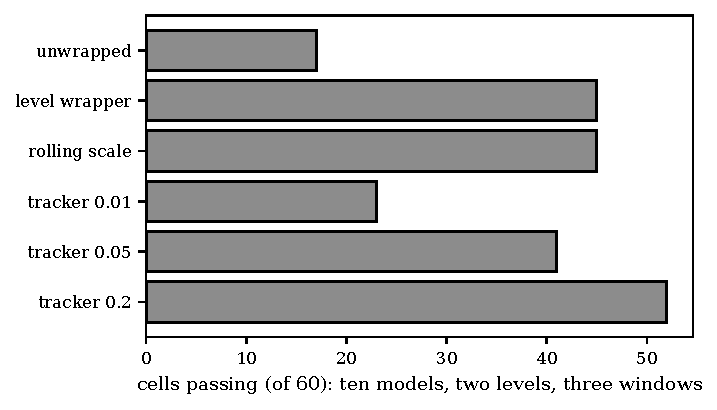
\includegraphics[width=0.62\textwidth]{methods-pass}
\caption{Cells passed (Kupiec and conditional coverage both at least 0.05) out of 60 by the unwrapped models, the level wrapper and four recalibrations of the finished value at risk, for the ten wrapped ladder models at two levels in the three stress windows.}
\label{fig:methods-pass}
\end{figure}

\subsection{Generators of known truth}
\label{sec:results-generators}

\Cref{tab:generators} and \cref{fig:generator-pass} give the generator study, with \genReps{} replications of each of four scenarios. With a shift, the wrapped pass rate is above the unwrapped one in all \genPredANum{} of \genPredADen{} model-level-scenario cells (prediction (a) held on the pass rates; \cref{sec:results-dispersion} shows how much of these differences the tests themselves produce). The unwrapped historical simulation passes in \genPassCrisisHsTwoFiftyOneUnw{} of replications of the persistent crisis at the 1\% level and the wrapped model in \genPassCrisisHsTwoFiftyOneAci{}; in the decaying crash the wrapped pass rate is \genPassCrashHsTwoFiftyOneAci{} for historical simulation at 1\%, the lowest of any shift cell (\genLowestAciPass{}, in \genLowestAciScen{}), which is prediction (d): the shortest window is repaired least. Prediction (c) held in \genPredCNum{} of the 18 cells with a shift, and (e) in \genPredENum{} of \genPredEDen{}: the wrapper lowers the mean error of the historical-simulation VaR against the true VaR in every scenario with a shift.

One prediction did not hold as stated. Prediction (b), that with no shift the wrapped pass rate is within 0.05 of the unwrapped one, held in \genPredBWithin{} of 6 cells: the wrapped pass rate is higher by \genPredBDiffMin{} to \genPredBDiffMax{}. The cause is not a mean hit rate off the target in the no-shift scenario: GARCH-t and FHS at the 1\% level have unwrapped mean hit rates of \genHitNullGarchTOneUnw\% and \genHitNullFhsOneUnw\%, on the target, and their pass rate still rises to \genPassNullGarchTOneAci{} and \genPassNullFhsOneAci{} once wrapped. Two properties of the counts raise it: the wrapped hit count is less variable than a binomial count and the tests accept it more easily, and the unwrapped counts of these two models are more variable than a binomial count, which lowers their own pass rate (\cref{sec:results-dispersion}); the mis-sizing of historical simulation at 1\% (a mean hit rate of \genHitNullHsTwoFiftyOneUnw\% in the control, a finite-sample understatement of the tail) is a second, partial cause for that model only. The second part of (b), a median score change within 2\%, held (largest \genPredBFzMax\%). A further negative result, which no prediction covered, concerns accuracy against the truth. For the two filtered models the wrapper raises the mean absolute log error of the VaR against the true VaR in \genErrWorseCells{} of \genErrWorseDen{} cells (four scenarios, two models, two levels): the fluctuation of the level adds noise to a VaR that the filter already tracks, so passes are gained at the price of VaR accuracy. The independence of the hits is not harmed in any generator cell: the share of replications with an independence p-value of at least 0.05 falls by at most \genIndDropMax{} (\cref{tab:generators}), a statement that carries the limit of the independence test discussed in \cref{sec:discussion-why}.

\begin{table*}[htbp]
\centering
\small
\caption{Generators of known truth, 100 replications per scenario: pass rate (Kupiec and conditional coverage both at least 0.05) of the unwrapped model and of three recalibrations, each with its 95\% Wilson interval; the mean absolute log error of the VaR against the true conditional VaR, unwrapped (U) and wrapped (W); and the median relative FZ0 change of the level wrapper.}
\label{tab:generators}
\begin{adjustbox}{max width=\textwidth}
\begin{tabular}{llrlllllr}
\toprule
Scenario & Model & Level (\%) & Unwrapped & Level wrapper & Rolling scale & Tracker & VaR error U / W & Median FZ0 change W \\
\midrule
No shift & HS-250 & 1 & 0.85 (0.77--0.91) & 0.99 (0.95--1.00) & 0.95 (0.89--0.98) & 0.93 (0.86--0.97) & 0.259 / 0.265 & \relax +0.2\% \\
No shift & HS-250 & 2.5 & 0.76 (0.67--0.83) & 0.94 (0.88--0.97) & 0.91 (0.84--0.95) & 0.91 (0.84--0.95) & 0.238 / 0.241 & \relax +0.1\% \\
No shift & GARCH-t & 1 & 0.85 (0.77--0.91) & 0.99 (0.95--1.00) & 0.99 (0.95--1.00) & 0.98 (0.93--0.99) & 0.051 / 0.107 & \relax +0.8\% \\
No shift & GARCH-t & 2.5 & 0.94 (0.88--0.97) & 1.00 (0.96--1.00) & 1.00 (0.96--1.00) & 1.00 (0.96--1.00) & 0.044 / 0.080 & \relax +0.4\% \\
No shift & FHS & 1 & 0.76 (0.67--0.83) & 0.99 (0.95--1.00) & 0.97 (0.92--0.99) & 0.92 (0.85--0.96) & 0.075 / 0.117 & \relax +0.6\% \\
No shift & FHS & 2.5 & 0.86 (0.78--0.91) & 1.00 (0.96--1.00) & 1.00 (0.96--1.00) & 1.00 (0.96--1.00) & 0.060 / 0.086 & \relax +0.4\% \\
Persistent crisis & HS-250 & 1 & 0.25 (0.18--0.34) & 0.92 (0.85--0.96) & 0.77 (0.68--0.84) & 0.73 (0.64--0.81) & 0.504 / 0.466 & \relax -9.4\% \\
Persistent crisis & HS-250 & 2.5 & 0.22 (0.15--0.31) & 0.96 (0.90--0.98) & 0.79 (0.70--0.86) & 0.80 (0.71--0.87) & 0.495 / 0.465 & \relax -6.5\% \\
Persistent crisis & GARCH-t & 1 & 0.62 (0.52--0.71) & 0.95 (0.89--0.98) & 0.97 (0.92--0.99) & 0.83 (0.74--0.89) & 0.177 / 0.166 & \relax +0.4\% \\
Persistent crisis & GARCH-t & 2.5 & 0.46 (0.37--0.56) & 0.99 (0.95--1.00) & 0.96 (0.90--0.98) & 0.92 (0.85--0.96) & 0.173 / 0.153 & \relax -0.1\% \\
Persistent crisis & FHS & 1 & 0.62 (0.52--0.71) & 0.95 (0.89--0.98) & 0.96 (0.90--0.98) & 0.84 (0.76--0.90) & 0.175 / 0.175 & \relax +0.8\% \\
Persistent crisis & FHS & 2.5 & 0.45 (0.36--0.55) & 0.99 (0.95--1.00) & 0.96 (0.90--0.98) & 0.94 (0.88--0.97) & 0.172 / 0.155 & \relax +0.2\% \\
Decaying crash & HS-250 & 1 & 0.26 (0.18--0.35) & 0.68 (0.58--0.76) & 0.26 (0.18--0.35) & 0.34 (0.25--0.44) & 0.460 / 0.451 & \relax -27.8\% \\
Decaying crash & HS-250 & 2.5 & 0.24 (0.17--0.33) & 0.81 (0.72--0.87) & 0.44 (0.35--0.54) & 0.39 (0.30--0.49) & 0.497 / 0.470 & \relax -14.1\% \\
Decaying crash & GARCH-t & 1 & 0.72 (0.63--0.80) & 0.93 (0.86--0.97) & 0.73 (0.64--0.81) & 0.78 (0.69--0.85) & 0.187 / 0.238 & \relax +1.9\% \\
Decaying crash & GARCH-t & 2.5 & 0.77 (0.68--0.84) & 0.96 (0.90--0.98) & 0.95 (0.89--0.98) & 0.90 (0.83--0.94) & 0.180 / 0.199 & \relax +0.1\% \\
Decaying crash & FHS & 1 & 0.70 (0.60--0.78) & 0.91 (0.84--0.95) & 0.72 (0.63--0.80) & 0.76 (0.67--0.83) & 0.198 / 0.243 & \relax +1.4\% \\
Decaying crash & FHS & 2.5 & 0.81 (0.72--0.87) & 0.98 (0.93--0.99) & 0.95 (0.89--0.98) & 0.94 (0.88--0.97) & 0.188 / 0.204 & \relax +0.1\% \\
Upward drift & HS-250 & 1 & 0.59 (0.49--0.68) & 0.97 (0.92--0.99) & 0.96 (0.90--0.98) & 0.77 (0.68--0.84) & 0.275 / 0.244 & \relax -2.2\% \\
Upward drift & HS-250 & 2.5 & 0.43 (0.34--0.53) & 0.95 (0.89--0.98) & 0.91 (0.84--0.95) & 0.66 (0.56--0.75) & 0.266 / 0.224 & \relax -1.4\% \\
Upward drift & GARCH-t & 1 & 0.87 (0.79--0.92) & 1.00 (0.96--1.00) & 0.98 (0.93--0.99) & 0.97 (0.92--0.99) & 0.117 / 0.131 & \relax +1.1\% \\
Upward drift & GARCH-t & 2.5 & 0.81 (0.72--0.87) & 1.00 (0.96--1.00) & 0.97 (0.92--0.99) & 0.98 (0.93--0.99) & 0.112 / 0.110 & \relax +0.3\% \\
Upward drift & FHS & 1 & 0.83 (0.74--0.89) & 0.99 (0.95--1.00) & 0.98 (0.93--0.99) & 0.93 (0.86--0.97) & 0.121 / 0.142 & \relax +0.8\% \\
Upward drift & FHS & 2.5 & 0.82 (0.73--0.88) & 0.99 (0.95--1.00) & 0.97 (0.92--0.99) & 0.96 (0.90--0.98) & 0.115 / 0.117 & \relax +0.4\% \\
\bottomrule
\end{tabular}
\end{adjustbox}
\end{table*}


\begin{figure}[htbp]
\centering
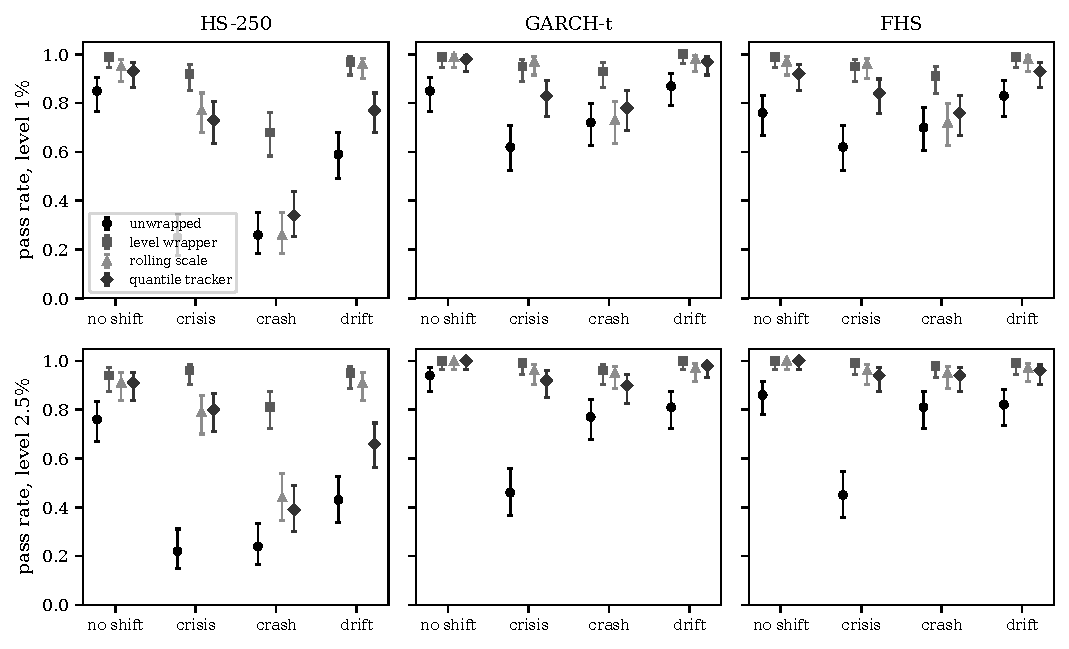
\includegraphics[width=\textwidth]{generator-pass}
\caption{Pass rate over 100 replications of each scenario for HS-250, GARCH-t and FHS at the 1\% (top) and 2.5\% (bottom) levels: the unwrapped model and three recalibrations, with 95\% Wilson intervals; the scenarios are no shift, a persistent crisis, a decaying crash and an upward drift of the volatility.}
\label{fig:generator-pass}
\end{figure}

\subsection{How easily the back-tests accept a wrapped run}
\label{sec:results-dispersion}

The no-shift scenario of the generators holds a result that the pass counts above cannot show. For GARCH-t and FHS at the 1\% level the unwrapped mean hit rate is \genHitNullGarchTOneUnw\% and \genHitNullFhsOneUnw\%, on the target, and the models pass in \genPassNullGarchTOneUnw{} and \genPassNullFhsOneUnw{} of the replications; the wrapped models pass in \genPassNullGarchTOneAci{} and \genPassNullFhsOneAci{} (\cref{tab:dispersion-null}). A mean on the target does not make these models right in each replication: the standard deviation of the unwrapped hit rate across replications is \dispSdNullGarchTOneUnw{} points for GARCH-t and \dispSdNullFhsOneUnw{} for FHS, against the binomial value of \dispBinNullGarchTOneUnw{} and \dispBinNullFhsOneUnw{} points for independent hits at that rate and that length (ratios \dispRatioNullGarchTOneUnw{} and \dispRatioNullFhsOneUnw{}), the estimation error of each replication, and their pass rates sit below the \dispBOneOneUnwPass\% of a model known to be correct (\cref{tab:dispersion}, $c = 1$). Part of the rise in the pass rate is therefore a repair of the coverage of each run, which the wrapper makes. The rest is the spread of the wrapped hit rate: its standard deviation falls to \dispSdNullGarchTOneAci{} points for GARCH-t and \dispSdNullFhsOneAci{} for FHS, below the binomial value. The wrapped hit count is under-dispersed. In the \dispRatioAciN{} model-level-scenario cells of the generators the ratio of the wrapped standard deviation to the binomial one runs from \dispRatioAciMin{} to \dispRatioAciMax{} (below one in \dispRatioAciBelow{} cells), for the rolling scale from \dispRatioRollMin{} to \dispRatioRollMax{} and for the quantile tracker from \dispRatioTrkMin{} to \dispRatioTrkMax{}, while for the unwrapped models it runs from \dispRatioUnwMin{} to \dispRatioUnwMax{}. This is the identity of \cref{prop:identity} at work: a hit lowers the level and a quiet day raises it, so the running count cannot wander far from its target, and the count is less variable than that of independent hits. The Kupiec and conditional coverage tests, and the Wilson interval of the hit rate, are built for independent hits; they accept a run whose count is held near the target more easily than its coverage warrants. In the no-shift scenario the pass rate of the wrapped models runs from \dispNullPassAciMin{} to \dispNullPassAciMax{}, that of the rolling scale from \dispNullPassRollMin{} to \dispNullPassRollMax{} and that of the tracker from \dispNullPassTrkMin{} to \dispNullPassTrkMax{}, against \dispNullPassUnwMin{} to \dispNullPassUnwMax{} for the unwrapped models. These ranges are not a measure of the size of the tests: the models of the scenario are estimated, not known, and HS-250 at the 2.5\% level has an unwrapped hit rate of \genHitNullHsTwoFiftyTwoHalfUnw\% against the target of 2.5\%. The size is measured next, on a model that is correct by construction.

\begin{table}[htbp]
\centering
\small
\caption{The control scenario (no shift, 500 days, 100 replications): the mean hit rate, the standard deviation of the hit rate across replications of the unwrapped (U) and wrapped (W) model against the binomial standard deviation at the unwrapped mean rate, and the pass rate of the unwrapped model and of three recalibrations.}
\label{tab:dispersion-null}
\begin{adjustbox}{max width=\textwidth}
\begin{tabular}{llrrr}
\toprule
Model & Level (\%) & Mean hit rate (\%) U / W & Hit-rate s.d. (points) U / W / binomial & Pass rate U / W / rolling / tracker \\
\midrule
HS-250 & 1 & 1.31 / 1.13 & 0.51 / 0.26 / 0.51 & 0.85 / 0.99 / 0.95 / 0.93 \\
HS-250 & 2.5 & 2.98 / 2.61 & 0.89 / 0.36 / 0.76 & 0.76 / 0.94 / 0.91 / 0.91 \\
GARCH-t & 1 & 1.01 / 1.01 & 0.52 / 0.22 / 0.45 & 0.85 / 0.99 / 0.99 / 0.98 \\
GARCH-t & 2.5 & 2.51 / 2.48 & 0.75 / 0.33 / 0.70 & 0.94 / 1.00 / 1.00 / 1.00 \\
FHS & 1 & 1.00 / 1.02 & 0.61 / 0.23 / 0.44 & 0.76 / 0.99 / 0.97 / 0.92 \\
FHS & 2.5 & 2.52 / 2.48 & 0.88 / 0.37 / 0.70 & 0.86 / 1.00 / 1.00 / 1.00 \\
\bottomrule
\end{tabular}
\end{adjustbox}
\end{table}


\Cref{tab:dispersion} measures the effect on runs whose coverage is wrong, with independent returns, a model that misjudges the scale by a known ratio $c$, and \dispBReps{} runs of \dispBDays{} days per row. With a correct model ($c = 1$) at the 1\% level the standard deviation of the wrapped count is \dispBOneOneAciCntSd{} against \dispBOneOneAciBinSd{} for independent hits; the Kupiec test rejects \dispBOneOneAciKupRej\% of the wrapped runs and \dispBOneOneUnwKupRej\% of the unwrapped runs, and the share of runs that pass both tests is \dispBOneOneAciPass\% against \dispBOneOneUnwPass\%. When the scale of the model is 1/1.25 of the scale of the data ($c = 1.25$) at the 1\% level, the true hit probability of the wrapped runs is \dispBOneOneTwoFiveAciTrueP\% against the target of 1\%, and the Kupiec test rejects \dispBOneOneTwoFiveAciKupRej\% of them, against \dispBOneOneTwoFiveAciRefKupRej\% of independent hits drawn at the same probability; \dispBOneOneTwoFiveAciPass\% of the wrapped runs pass, against \dispBOneOneTwoFiveAciRefPass\% for the independent reference. At the 2.5\% level the same error leaves a true hit probability of \dispBTwoHalfOneTwoFiveAciTrueP\% and a Kupiec rejection of \dispBTwoHalfOneTwoFiveAciKupRej\% against \dispBTwoHalfOneTwoFiveAciRefKupRej\% for the reference. The gap to the independent reference closes only at the larger errors: at the 1\% level the Kupiec test rejects \dispBOneOneFiveAciKupRej\% of the wrapped runs at $c = 1.5$ against \dispBOneOneFiveAciRefKupRej\% for the reference, and \dispBOneTwoAciKupRej\% against \dispBOneTwoAciRefKupRej\% at $c = 2$; at the 2.5\% level it is still open at $c = 1.5$ (\dispBTwoHalfOneFiveAciKupRej\% against \dispBTwoHalfOneFiveAciRefKupRej\%) and closed at $c = 2$ (\dispBTwoHalfTwoAciKupRej\% against \dispBTwoHalfTwoAciRefKupRej\%). At the errors where it closes the wrapped runs are far from the target and the wrapper has also stopped repairing. The Wilson interval of the hit rate contains the true hit probability of the run in \dispWilsonMin\% to \dispWilsonMax\% of the runs in every row, so the intervals of the figures describe the realised hit rate correctly; it is the decision of the tests, and the counts of passes built on them, that are too lenient.

\begin{table}[htbp]
\centering
\small
\caption{The back-tests on wrapped runs whose model misjudges the scale by the ratio $c$ ($c = 1$: a correct model), 4,000 independent runs of 500 days per row. The true hit probability is the mean over the days of the probability that the loss exceeds the VaR at that day's level; the count s.d. is the standard deviation of the hit count of the wrapped runs against the binomial one at that probability. Kupiec rejection is the share of runs with a Kupiec p-value below 0.05 (a run with no hit has one, and it rejects) for the unwrapped runs (U), the wrapped runs (W) and independent Bernoulli hits drawn at the wrapped true probability (iid, the reference the test assumes); pass is the share with Kupiec and conditional coverage both at least 0.05 (a run with no hit has no conditional coverage p-value and does not pass).}
\label{tab:dispersion}
\begin{adjustbox}{max width=\textwidth}
\begin{tabular}{lrrrrr}
\toprule
Level (\%) & Scale ratio $c$ & True hit probability (\%) U / W & Count s.d. W / binomial & Kupiec rejection (\%) U / W / iid & Pass (\%) U / W / iid \\
\midrule
1 & 0.75 & 0.32 / 0.57 & 1.17 / 1.69 & 53.4 / 12.0 / 23.4 & 46.3 / 87.5 / 76.0 \\
1 & 1 & 1.00 / 1.01 & 1.05 / 2.23 & 7.1 / 0.1 / 7.6 & 92.6 / 99.8 / 91.8 \\
1 & 1.25 & 2.16 / 1.36 & 1.20 / 2.59 & 63.2 / 2.3 / 14.4 & 36.7 / 97.5 / 85.5 \\
1 & 1.5 & 3.75 / 1.80 & 1.64 / 2.97 & 98.8 / 34.3 / 40.0 & 1.2 / 65.6 / 59.7 \\
1 & 2 & 7.67 / 3.09 & 2.75 / 3.87 & 100.0 / 99.3 / 94.4 & 0.0 / 0.7 / 5.6 \\
2.5 & 0.75 & 0.93 / 1.60 & 1.78 / 2.80 & 81.3 / 20.2 / 32.3 & 17.9 / 78.0 / 66.4 \\
2.5 & 1 & 2.50 / 2.51 & 1.55 / 3.50 & 6.2 / 0.0 / 6.7 & 92.9 / 99.5 / 92.5 \\
2.5 & 1.25 & 4.74 / 3.05 & 1.25 / 3.85 & 80.0 / 0.0 / 15.4 & 19.8 / 99.6 / 83.9 \\
2.5 & 1.5 & 7.36 / 3.41 & 1.38 / 4.06 & 99.9 / 4.9 / 26.8 & 0.1 / 93.9 / 72.4 \\
2.5 & 2 & 12.75 / 4.61 & 2.63 / 4.69 & 100.0 / 92.0 / 77.0 & 0.0 / 7.9 / 22.5 \\
\bottomrule
\end{tabular}
\end{adjustbox}
\end{table}


The pass counts of the ten models can be recomputed against this. The Kupiec test is replaced by a two-sided exact test on the hit count, with the binomial distribution as the null of an unwrapped run and, as the null of a wrapped run, the distribution of the count of \dispCNullReps{} simulated wrapped runs of a correct model of the same length and level (standard deviation of the wrapped null count \dispCNullSdEqCrisisOne{} at the 1\% level in the financial crisis window against \dispCBinSdEqCrisisOne{} binomial). The independence part of the conditional coverage test is not recalibrated, so this is a test of coverage only. Of the \dispCCells{} cells the unwrapped models pass \dispCUnwExact{} (the engine's asymptotic Kupiec test gives \dispCUnwAsy{}) and the wrapped models pass \dispCWrapCal{} (\dispCWrapAsy{} by the engine's test; \dispCWrapExact{} by the binomial test, so \dispCFlips{} cells change status once the wrapped count is tested against its own null). The gain in cells passed is therefore \dispCWrapCal{} against \dispCUnwExact{}, not \tenPassAci{} against \tenPassUnw{}. For the three models of H1, the wrapped models pass \dispCHoneWrap{} of \dispCHoneCells{} cells and the unwrapped \dispCHoneUnw{}, and H1 holds in \dispCHoneGainCal{} of its \hypCells{} cells on coverage alone (the cell that no longer holds is \dispCHoneLost). The null of this recomputation is a correct model on independent returns; it is the reference for a size, not a model of the real windows, whose wrapped counts also depend on the misspecification of each model.

What survives is the movement of the hit rate and the score. The mean distance of the hit rate from its target falls from \tenHitDevUnw{} to \tenHitDevAci{} points, the hit rate of the wrapped run is closer to the target than the unwrapped one in every shift scenario of the generators (prediction (c)), the error of the HS-250 VaR against the truth falls in every shift scenario (prediction (e)), and the change of the score is as reported. What does not survive is the size of the gain in passes: a model that is correct by construction passes in \dispBOneOneAciPass\% of the wrapped runs against \dispBOneOneUnwPass\% of the unwrapped runs at the 1\% level, and in \dispBTwoHalfOneAciPass\% against \dispBTwoHalfOneUnwPass\% at the 2.5\% level, so a difference of that size carries no information on coverage. The wider gap of the no-shift scenario (\dispNullPassAciMin{} to \dispNullPassAciMax{} against \dispNullPassUnwMin{} to \dispNullPassUnwMax{}) is partly the same leniency and partly the over-dispersion of the unwrapped estimated models themselves, which the wrapper legitimately reduces. The pass rates of the shift scenarios are upper bounds. In the persistent crisis the wrapped historical simulation passes in \genPassCrisisHsTwoFiftyOneAci{} of the replications at the 1\% level while its mean hit rate is \genHitCrisisHsTwoFiftyOneAci\% against the target of 1\%.
